\section{Engine and Transmission}

The electronic hardware for the engine and transmission module was completely constructed and debugged. Additionally, all of the software sub-components were constructed. Full testing of the system software on the engine and transmission module was not possible since a pneumatic system prototype was unavailable, and the car not yet constructed. Completion of this stage of the implementation is recommended for future work.

\subsection{Electro-pneumatic Simulation}

The electro-pneumatic Simulink model as described in Sec.\ \ref{sec:electropneumatic_implementation} was simulated by feeding the closed-loop system with a reference input representing 50\% of the maximum travel of the clutch. Figure \ref{fig:pneumatic_sim} shows the closed-loop response to the step input, recorded until the output stabilized. Figure \ref{fig:pneumatic_sim_zoom} shows a close up view of the first peak in the response, detailing the result of the compressibility effects of the air in the cylinder. The PID controller block was minimally tuned only until a stable response was obtained.

\begin{figure}[H]
 \centering
 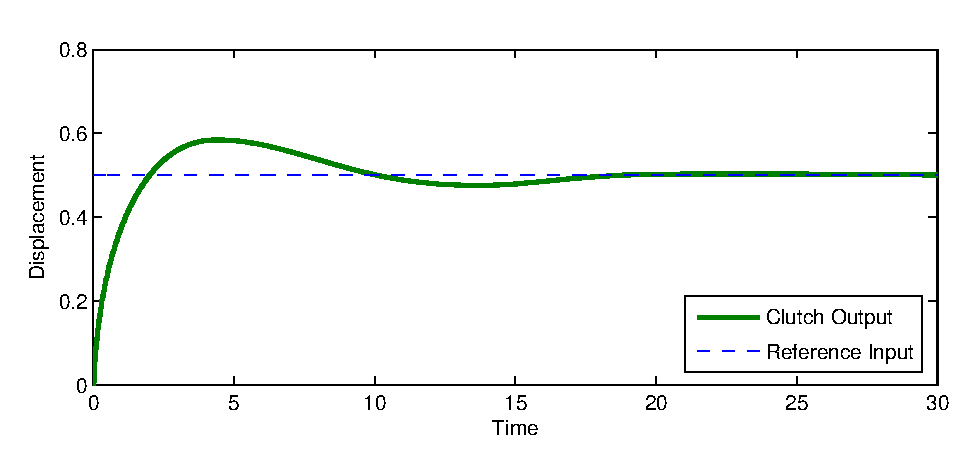
\includegraphics[width=5in,keepaspectratio]{results/figures/electro-pneumatic_simulation_plot.eps}
 \caption{Simulink output of the electro-pneumatic simulation.}
 \label{fig:pneumatic_sim}
\end{figure}

The point of the simulation was to verify the feasibility of closed-loop control over the electro-pneumatic system in the configuration proposed. It is important to note that correct model parameters corresponding to the real physical pneumatic valves, cylinders, clutch, etc., were not obtained.

\begin{figure}[H]
 \centering
 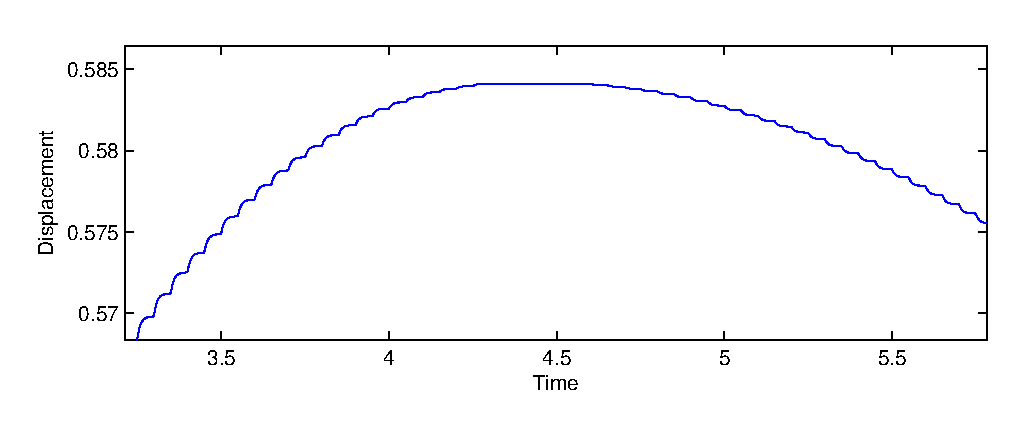
\includegraphics[width=5in,keepaspectratio]{results/figures/electro-pneumatic_simulation_plot2.eps}
 \caption{Close-up of the peak response of the electro-pneumatic simulation.}
 \label{fig:pneumatic_sim_zoom}
\end{figure}

\section{Intake}

As of writing, the Formula SAE team members responsible for designing and implementing the two stage intake-plenum were still in the design stages of that project. Our contributions to the variable intake-plenum project, namely the electronics to provide the control signal from the engine and transmission module, are complete. Completing the control software and testing this system will need to be done after the intake is fully designed and manufactured.
